\chapter{DualPipe}

\section{Introduction}
\subsection{All-to-All vs Point-to-Point}
% \label{sec:}

When orchestrating multiple GPUs, we need them to communicate with each other to share information like gradients and model parameters. There are two main types of communication patterns: 
\begin{enumerate}
	\item All-to-all communication.
	\item Point-to-point communication.
\end{enumerate}

\textit{All-to-all communication} involves every GPU in the system simultaneously exchanging data with all other GPUs. The canonical analogy is a group chat where everyone needs to share their updates with everyone else. All-to-all communication is expensive and involves a ton of communication overhead. There are several clever algorithms like ring-AllReduce that can reduce this overhead, but it's still often a bottleneck.

\textit{Point-to-point communication}, on the other hand, is a communication between just two GPUs (the analogy here is a private conversation). One GPU sends data directly to another specific GPU without involving the rest of the system. This is much more efficient in terms of network bandwidth and latency. In practice, point-to-point communication is strongly preferred when possible because it's significantly cheaper in terms of computational resources.



\section{DualPipe}

\begin{figure}[t]
	\centering
	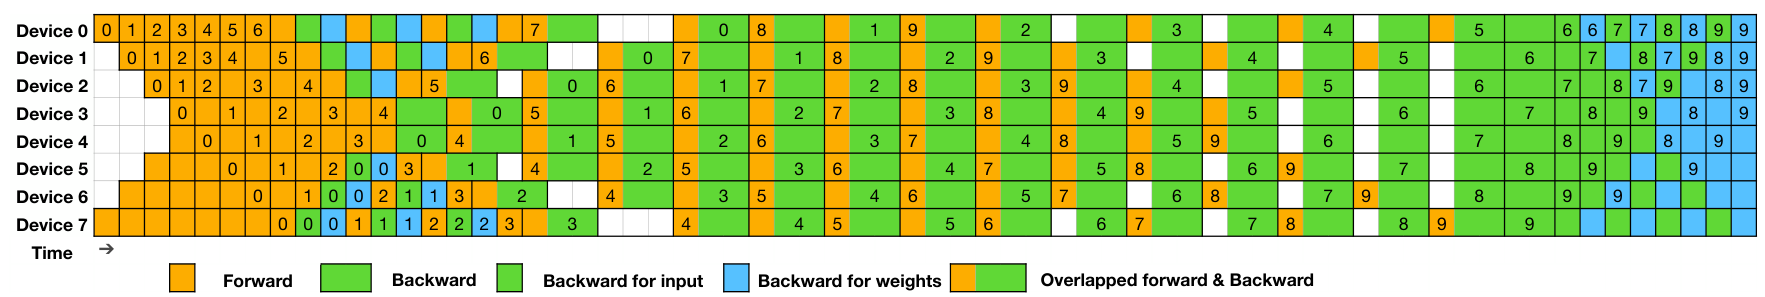
\includegraphics[scale=0.45]{./images/dualpipe.png}
	\caption{An illustration of dualpipe.}
\end{figure}
Finer-Grained stages: divide each chunk into 4 components: 
\begin{itemize}
	\item Attention, 
	\item All-to-all dispatch(Handles communication between devices), 
	\item MLP(Multi-Layer Perceptron), 
	\item All-to-all combine(merge output across devices).
\end{itemize}
 For a backward chunk, the attention and MLP split further into two parts: backward for input($B$) and backward for weights($W$) like Zero Bubble.

Bidirectional pipeline scheduling which feeds micro-batches from both ends of the pipeline simultaneously and a significant portion of communications can be fully overlapped (See the 2 black arrows in following diagram). In order to support bidirectional pipeline scheduling, DualPipe requires keeping two copies of the model parameters. If we have 8 devices with a 8 layers model, in the Zero Bubble Schedule, each device has a corresponding layer. But in the DualPipe Schedule, in order to handle bidirectional pipeline, the device 0 should have model's layer0 and layer7, and the device 7 should have model's layer7 and layer0.

